\documentclass[14pt,a4paper]{scrartcl}
\usepackage{cmap}
\usepackage[utf8]{inputenc}
\usepackage[T1,T2A]{fontenc}
\usepackage[english,russian]{babel}
\usepackage{relsize}
\usepackage{graphicx}
\usepackage{subfigure}
\usepackage{mathtools}
\usepackage{amssymb}
\usepackage{float}
\usepackage{sidecap}
\usepackage{wrapfig}
\usepackage{caption}
\usepackage[table,xcdraw]{xcolor}
\usepackage{listings}
\usepackage{amsmath,cryptocode}
\usepackage{listings}
\usepackage{booktabs}
\usepackage{multirow}  
\usepackage{multicol}
\usepackage{bigstrut}
\usepackage{lscape}
\usepackage{rotating}
\usepackage{adjustbox}
\usepackage{minted}
\usepackage{breqn}
\usepackage{physics}


\newcommand\scalemath[2]{\scalebox{#1}{\mbox{\ensuremath{\displaystyle #2}}}}


\begin{document}
	\begin{titlepage}
	\begin{center}
		\large
		МИНИСТЕРСТВО ОБРАЗОВАНИЯ И НАУКИ\\ РОССИЙСКОЙ ФЕДЕРАЦИИ
		
		\vspace{0.5cm}
		
		МГТУ им Н.Э.Баумана
		\vspace{0.25cm}
		
		Факультет ФН
		
		Кафедра вычислительной математики и математической физики
		\vfill
		
		
		Соколов Арсений Андреевич\\
		\vfill
		
		
		{\LARGE Лабораторная работа №7 по численным методам\\[2mm]
		}
		\bigskip
		
		3 курс, группа ФН11-53Б\\
		Вариант 6
	\end{center}
	\vfill
	
	\newlength{\ML}
	\settowidth{\ML}{«\underline{\hspace{0.7cm}}» \underline{\hspace{2cm}}}
	\hfill\begin{minipage}{0.4\textwidth}
		Преподаватель\\
		\underline{\hspace{3cm}} В.\,А.~Кутыркин\\
		«\underline{\hspace{0.7cm}}» \underline{\hspace{1.71cm}} 2019 г.
	\end{minipage}%
	\bigskip
	
	
	\vfill
	
	\begin{center}
		Москва, 2019 г.
	\end{center}
\end{titlepage}

\section*{Задание 1}
\textbf{Задание.}\\
Используя дискретный аналог уравнения (1) Фредгольма 2-го рода с симметричным, непрерывным и аналитически заданным ядром
\begin{equation}
	x(s)-\lambda \int_{a}^{b} K(s, \tau) x(\tau) d \tau=y(s), \quad s \in[a ; b]
\end{equation}
индуцированный методом конечных сумм с квадратурными формулами прямоугольников (количество узлов в квадратурной формуле не менее 20), найти приближённое решение уравнения (1), которое имеет конкретный вид:
\begin{equation*}
	x(s)-\frac{1}{n-49} \int_{0}^{\frac{N+5}{\mu}} K(s, \tau) x(\tau) d \tau=\frac{N+5}{N}\left(s^{2}+n-49\right), \quad s \in\left[0 ; \frac{N+5}{N}\right]
\end{equation*}

(N -- номер студента в журнале, n -- номер группы)
И
\begin{equation*}
	K(s, \tau)=\left\{\begin{array}{ll}{s\left(2 \frac{N+5}{N}-\tau\right),} & {0 \leq s \leq \tau} \\ {\tau\left(2 \frac{N+5}{N}-s\right),} & {\tau \leq s \leq \frac{N+5}{N}}\end{array}\right.
\end{equation*}

Оценить абсолютную погрешность приближённого решения, сравнив его с аналитическим решением, полученным сведением уравнения (1) к краевой
задаче для обыкновенного линейного дифференциального уравнения 2-го порядка с постоянными коэффициентами.\\

\textbf{Исходные данные.}\\
$N = 6, n = 53$


\textbf{Решение.}\\
Будем использовать 20 узлов. Для построения дискретного аналога, аппроксимирующего уравнение (1), зададим на квадрате $[0; \frac{11}{6}]\times[0;\frac{11}{6}]$ двумерную центрально-равномерную сетку $B \times A=\left\langle\left(s_{i}, \tau_{i}\right): s_{i} \in B, \tau_{i} \in A\right\rangle$ типа $20 \times 20$ шага $(h, \tau)$. Следовательно,  $B =\left\langle s_1, s_2, \ldots s_{20}\right\rangle$ и $A =\left\langle \tau_1, \tau_2, \ldots \tau_{20}\right\rangle$ центрально равномерные сетки отрезка $[0;\frac{11}{6}]\times[0;\frac{11}{6}]$ с шагами $h = \frac{b-a}{n} = \frac{11}{120}$ и $\tau = \frac{b-a}{n} = \frac{11}{120}$, соответственно.\\
Получим:
\begin{align*}
	&A = B = \\
	& \left\langle
	{\frac{11}{80}},
	{\frac{11}{48}},
	{\frac{77}{240}},
	{\frac{33}{80}},
	{\frac{121}{240}},
	{\frac{143}{240}},
	{\frac{11}{16}},
	{\frac{187}{240}},
	{\frac{209}{240}},
	{\frac{77}{80}},
	{\frac{253}{240}},
	{\frac{55}{48}},
	{\frac{99}{80}},
	{\frac{319}{240}},
	{\frac{341}{240}},
	{\frac{121}{80}},
	{\frac{77}{48}},
	{\frac{407}{240}},
	{\frac{143}{80}}\right\rangle
\end{align*}

Для любого узла $(s_i,\tau_i) \in B\times A \quad (i,j = \overline{1,20})$ и функций $K,x,y$ из уравнения
(1) приняты обозначения: $K_{j}^{i}=K(s_{i} ; \tau_{j}), \quad x^{j}=x\left(\tau_{j}\right)=x\left(s_{j}\right).$ и ${y^i = y(s_i)}$. Используя эти обозначения и квадратурную формулу прямоугольников, из уравнения (1) получаем его дискретный аналог, аппроксимирующий уравнение (1) при $h, \tau \rightarrow 0$, в виде СЛАУ 
\begin{equation*}
	K(s, \tau)=\left\{\begin{array}{l}{x^{i}-\lambda \sum_{j=1}^{20} K_{j}^{i} h \cdot x_{j}=y^{i}} \\ {i=\overline{1,20}}\end{array}\right.
\end{equation*}
Введём обозначения:
\begin{equation*}
	^>x=\left[x^{1}, \ldots, x^{20}\right\rangle,^>y=\left[y^{1}, \ldots, y^{20}\right\rangle \in ^>R^{n}, F=\left(\delta_{j}^{i}-\lambda K_{j}^{i} \cdot h\right)_{20}^{20}=\left(f_{j}^{i}\right)_{20}^{20} \in L(R, 20),
\end{equation*}
где
\begin{equation*}
	\delta_{j}^{i}=\left\{\begin{array}{l}{1, i=j} \\ {0, i \neq j}\end{array}\right.
\end{equation*}

Используя эти обозначения, СЛАУ перепишем в виде $F\cdot ^>x = ^>y$.

Найдём приближенное решение уравнения
\begin{equation*}
	x(s)-\frac{1}{4} \int_{0}^{\frac{11}{6}} K(s, \tau) x(\tau) d \tau=\frac{11}{6}\left(s^{2}+4\right), \quad s \in[0 ; \frac{11}{6}]
\end{equation*}

\begin{equation*}
	K(s, \tau)=\left\{\begin{array}{ll}{s(\frac{11}{3}-\tau),} & {0 \leq s \leq \tau} \\ {\tau(\frac{11}{3}-s),} & {\tau \leq s \leq \frac{11}{3}}\end{array}\right.
\end{equation*}

Так как $F\cdot ^>x = ^>y$, следовательно $^>x = F^-1 \cdot ^>y$.\\
Необходимые вычисления :
\begin{align*}
\resizebox{1.1 \textwidth}{!} 
{$F =  \left[ \begin {array}{cccccccccccccccccccc} {\frac{27542851}{27648000
}}&-{\frac{102487}{27648000}}&-{\frac{1331}{368640}}&-{\frac{97163}{
		27648000}}&-{\frac{94501}{27648000}}&-{\frac{30613}{9216000}}&-{\frac{
		89177}{27648000}}&-{\frac{17303}{5529600}}&-{\frac{9317}{3072000}}&-{
	\frac{81191}{27648000}}&-{\frac{78529}{27648000}}&-{\frac{25289}{
		9216000}}&-{\frac{14641}{5529600}}&-{\frac{70543}{27648000}}&-{\frac{
		22627}{9216000}}&-{\frac{65219}{27648000}}&-{\frac{62557}{27648000}}&-
{\frac{1331}{614400}}&-{\frac{57233}{27648000}}&-{\frac{54571}{
		27648000}}\\ \noalign{\medskip}-{\frac{102487}{27648000}}&{\frac{
		9113513}{9216000}}&-{\frac{1331}{122880}}&-{\frac{97163}{9216000}}&-{
	\frac{94501}{9216000}}&-{\frac{30613}{3072000}}&-{\frac{89177}{9216000
}}&-{\frac{17303}{1843200}}&-{\frac{9317}{1024000}}&-{\frac{81191}{
		9216000}}&-{\frac{78529}{9216000}}&-{\frac{25289}{3072000}}&-{\frac{
		14641}{1843200}}&-{\frac{70543}{9216000}}&-{\frac{22627}{3072000}}&-{
	\frac{65219}{9216000}}&-{\frac{62557}{9216000}}&-{\frac{1331}{204800}}
&-{\frac{57233}{9216000}}&-{\frac{54571}{9216000}}
\\ \noalign{\medskip}-{\frac{1331}{368640}}&-{\frac{1331}{122880}}&{
	\frac{72397}{73728}}&-{\frac{97163}{5529600}}&-{\frac{94501}{5529600}}
&-{\frac{30613}{1843200}}&-{\frac{89177}{5529600}}&-{\frac{17303}{
		1105920}}&-{\frac{9317}{614400}}&-{\frac{81191}{5529600}}&-{\frac{
		78529}{5529600}}&-{\frac{25289}{1843200}}&-{\frac{14641}{1105920}}&-{
	\frac{70543}{5529600}}&-{\frac{22627}{1843200}}&-{\frac{65219}{5529600
}}&-{\frac{62557}{5529600}}&-{\frac{1331}{122880}}&-{\frac{57233}{
		5529600}}&-{\frac{54571}{5529600}}\\ \noalign{\medskip}-{\frac{97163}{
		27648000}}&-{\frac{97163}{9216000}}&-{\frac{97163}{5529600}}&{\frac{
		26967859}{27648000}}&-{\frac{661507}{27648000}}&-{\frac{214291}{
		9216000}}&-{\frac{624239}{27648000}}&-{\frac{121121}{5529600}}&-{\frac
	{65219}{3072000}}&-{\frac{568337}{27648000}}&-{\frac{549703}{27648000}
}&-{\frac{177023}{9216000}}&-{\frac{102487}{5529600}}&-{\frac{493801}{
		27648000}}&-{\frac{158389}{9216000}}&-{\frac{456533}{27648000}}&-{
	\frac{437899}{27648000}}&-{\frac{9317}{614400}}&-{\frac{400631}{
		27648000}}&-{\frac{381997}{27648000}}\\ \noalign{\medskip}-{\frac{
		94501}{27648000}}&-{\frac{94501}{9216000}}&-{\frac{94501}{5529600}}&-{
	\frac{661507}{27648000}}&{\frac{2977499}{3072000}}&-{\frac{30613}{
		1024000}}&-{\frac{89177}{3072000}}&-{\frac{17303}{614400}}&-{\frac{
		27951}{1024000}}&-{\frac{81191}{3072000}}&-{\frac{78529}{3072000}}&-{
	\frac{25289}{1024000}}&-{\frac{14641}{614400}}&-{\frac{70543}{3072000}
}&-{\frac{22627}{1024000}}&-{\frac{65219}{3072000}}&-{\frac{62557}{
		3072000}}&-{\frac{3993}{204800}}&-{\frac{57233}{3072000}}&-{\frac{
		54571}{3072000}}\\ \noalign{\medskip}-{\frac{30613}{9216000}}&-{\frac{
		30613}{3072000}}&-{\frac{30613}{1843200}}&-{\frac{214291}{9216000}}&-{
	\frac{30613}{1024000}}&{\frac{8879257}{9216000}}&-{\frac{980947}{
		27648000}}&-{\frac{190333}{5529600}}&-{\frac{102487}{3072000}}&-{\frac
	{893101}{27648000}}&-{\frac{863819}{27648000}}&-{\frac{278179}{9216000
}}&-{\frac{161051}{5529600}}&-{\frac{775973}{27648000}}&-{\frac{248897
	}{9216000}}&-{\frac{717409}{27648000}}&-{\frac{688127}{27648000}}&-{
	\frac{14641}{614400}}&-{\frac{629563}{27648000}}&-{\frac{600281}{
		27648000}}\\ \noalign{\medskip}-{\frac{89177}{27648000}}&-{\frac{89177
	}{9216000}}&-{\frac{89177}{5529600}}&-{\frac{624239}{27648000}}&-{
	\frac{89177}{3072000}}&-{\frac{980947}{27648000}}&{\frac{26488699}{
		27648000}}&-{\frac{224939}{5529600}}&-{\frac{121121}{3072000}}&-{\frac
	{1055483}{27648000}}&-{\frac{1020877}{27648000}}&-{\frac{328757}{
		9216000}}&-{\frac{190333}{5529600}}&-{\frac{917059}{27648000}}&-{\frac
	{294151}{9216000}}&-{\frac{847847}{27648000}}&-{\frac{813241}{27648000
}}&-{\frac{17303}{614400}}&-{\frac{744029}{27648000}}&-{\frac{709423}{
		27648000}}\\ \noalign{\medskip}-{\frac{17303}{5529600}}&-{\frac{17303}
	{1843200}}&-{\frac{17303}{1105920}}&-{\frac{121121}{5529600}}&-{\frac{
		17303}{614400}}&-{\frac{190333}{5529600}}&-{\frac{224939}{5529600}}&{
	\frac{351337}{368640}}&-{\frac{9317}{204800}}&-{\frac{81191}{1843200}}
&-{\frac{78529}{1843200}}&-{\frac{25289}{614400}}&-{\frac{14641}{
		368640}}&-{\frac{70543}{1843200}}&-{\frac{22627}{614400}}&-{\frac{
		65219}{1843200}}&-{\frac{62557}{1843200}}&-{\frac{1331}{40960}}&-{
	\frac{57233}{1843200}}&-{\frac{54571}{1843200}}\\ \noalign{\medskip}-{
	\frac{9317}{3072000}}&-{\frac{9317}{1024000}}&-{\frac{9317}{614400}}&-
{\frac{65219}{3072000}}&-{\frac{27951}{1024000}}&-{\frac{102487}{
		3072000}}&-{\frac{121121}{3072000}}&-{\frac{9317}{204800}}&{\frac{
		2913611}{3072000}}&-{\frac{1380247}{27648000}}&-{\frac{1334993}{
		27648000}}&-{\frac{429913}{9216000}}&-{\frac{248897}{5529600}}&-{\frac
	{1199231}{27648000}}&-{\frac{384659}{9216000}}&-{\frac{1108723}{
		27648000}}&-{\frac{1063469}{27648000}}&-{\frac{22627}{614400}}&-{\frac
	{972961}{27648000}}&-{\frac{927707}{27648000}}\\ \noalign{\medskip}-{
	\frac{81191}{27648000}}&-{\frac{81191}{9216000}}&-{\frac{81191}{
		5529600}}&-{\frac{568337}{27648000}}&-{\frac{81191}{3072000}}&-{\frac{
		893101}{27648000}}&-{\frac{1055483}{27648000}}&-{\frac{81191}{1843200}
}&-{\frac{1380247}{27648000}}&{\frac{26105371}{27648000}}&-{\frac{
		1492051}{27648000}}&-{\frac{480491}{9216000}}&-{\frac{278179}{5529600}
}&-{\frac{1340317}{27648000}}&-{\frac{429913}{9216000}}&-{\frac{
		1239161}{27648000}}&-{\frac{1188583}{27648000}}&-{\frac{25289}{614400}
}&-{\frac{1087427}{27648000}}&-{\frac{1036849}{27648000}}
\\ \noalign{\medskip}-{\frac{78529}{27648000}}&-{\frac{78529}{9216000}
}&-{\frac{78529}{5529600}}&-{\frac{549703}{27648000}}&-{\frac{78529}{
		3072000}}&-{\frac{863819}{27648000}}&-{\frac{1020877}{27648000}}&-{
	\frac{78529}{1843200}}&-{\frac{1334993}{27648000}}&-{\frac{1492051}{
		27648000}}&{\frac{8666297}{9216000}}&-{\frac{177023}{3072000}}&-{\frac
	{102487}{1843200}}&-{\frac{493801}{9216000}}&-{\frac{158389}{3072000}}
&-{\frac{456533}{9216000}}&-{\frac{437899}{9216000}}&-{\frac{9317}{
		204800}}&-{\frac{400631}{9216000}}&-{\frac{381997}{9216000}}
\\ \noalign{\medskip}-{\frac{25289}{9216000}}&-{\frac{25289}{3072000}}
&-{\frac{25289}{1843200}}&-{\frac{177023}{9216000}}&-{\frac{25289}{
		1024000}}&-{\frac{278179}{9216000}}&-{\frac{328757}{9216000}}&-{\frac{
		25289}{614400}}&-{\frac{429913}{9216000}}&-{\frac{480491}{9216000}}&-{
	\frac{177023}{3072000}}&{\frac{8634353}{9216000}}&-{\frac{336743}{
		5529600}}&-{\frac{1622489}{27648000}}&-{\frac{520421}{9216000}}&-{
	\frac{1500037}{27648000}}&-{\frac{1438811}{27648000}}&-{\frac{30613}{
		614400}}&-{\frac{1316359}{27648000}}&-{\frac{1255133}{27648000}}
\\ \noalign{\medskip}-{\frac{14641}{5529600}}&-{\frac{14641}{1843200}}
&-{\frac{14641}{1105920}}&-{\frac{102487}{5529600}}&-{\frac{14641}{
		614400}}&-{\frac{161051}{5529600}}&-{\frac{190333}{5529600}}&-{\frac{
		14641}{368640}}&-{\frac{248897}{5529600}}&-{\frac{278179}{5529600}}&-{
	\frac{102487}{1843200}}&-{\frac{336743}{5529600}}&{\frac{206543}{
		221184}}&-{\frac{70543}{1105920}}&-{\frac{22627}{368640}}&-{\frac{
		65219}{1105920}}&-{\frac{62557}{1105920}}&-{\frac{1331}{24576}}&-{
	\frac{57233}{1105920}}&-{\frac{54571}{1105920}}\\ \noalign{\medskip}-{
	\frac{70543}{27648000}}&-{\frac{70543}{9216000}}&-{\frac{70543}{
		5529600}}&-{\frac{493801}{27648000}}&-{\frac{70543}{3072000}}&-{\frac{
		775973}{27648000}}&-{\frac{917059}{27648000}}&-{\frac{70543}{1843200}}
&-{\frac{1199231}{27648000}}&-{\frac{1340317}{27648000}}&-{\frac{
		493801}{9216000}}&-{\frac{1622489}{27648000}}&-{\frac{70543}{1105920}}
&{\frac{953457}{1024000}}&-{\frac{67881}{1024000}}&-{\frac{65219}{
		1024000}}&-{\frac{62557}{1024000}}&-{\frac{11979}{204800}}&-{\frac{
		57233}{1024000}}&-{\frac{54571}{1024000}}\\ \noalign{\medskip}-{\frac{
		22627}{9216000}}&-{\frac{22627}{3072000}}&-{\frac{22627}{1843200}}&-{
	\frac{158389}{9216000}}&-{\frac{22627}{1024000}}&-{\frac{248897}{
		9216000}}&-{\frac{294151}{9216000}}&-{\frac{22627}{614400}}&-{\frac{
		384659}{9216000}}&-{\frac{429913}{9216000}}&-{\frac{158389}{3072000}}&
-{\frac{520421}{9216000}}&-{\frac{22627}{368640}}&-{\frac{67881}{
		1024000}}&{\frac{8559817}{9216000}}&-{\frac{1891351}{27648000}}&-{
	\frac{1814153}{27648000}}&-{\frac{38599}{614400}}&-{\frac{1659757}{
		27648000}}&-{\frac{1582559}{27648000}}\\ \noalign{\medskip}-{\frac{
		65219}{27648000}}&-{\frac{65219}{9216000}}&-{\frac{65219}{5529600}}&-{
	\frac{456533}{27648000}}&-{\frac{65219}{3072000}}&-{\frac{717409}{
		27648000}}&-{\frac{847847}{27648000}}&-{\frac{65219}{1843200}}&-{\frac
	{1108723}{27648000}}&-{\frac{1239161}{27648000}}&-{\frac{456533}{
		9216000}}&-{\frac{1500037}{27648000}}&-{\frac{65219}{1105920}}&-{\frac
	{65219}{1024000}}&-{\frac{1891351}{27648000}}&{\frac{25626211}{
		27648000}}&-{\frac{1939267}{27648000}}&-{\frac{41261}{614400}}&-{\frac
	{1774223}{27648000}}&-{\frac{1691701}{27648000}}\\ \noalign{\medskip}-
{\frac{62557}{27648000}}&-{\frac{62557}{9216000}}&-{\frac{62557}{
		5529600}}&-{\frac{437899}{27648000}}&-{\frac{62557}{3072000}}&-{\frac{
		688127}{27648000}}&-{\frac{813241}{27648000}}&-{\frac{62557}{1843200}}
&-{\frac{1063469}{27648000}}&-{\frac{1188583}{27648000}}&-{\frac{
		437899}{9216000}}&-{\frac{1438811}{27648000}}&-{\frac{62557}{1105920}}
&-{\frac{62557}{1024000}}&-{\frac{1814153}{27648000}}&-{\frac{1939267}
	{27648000}}&{\frac{8527873}{9216000}}&-{\frac{14641}{204800}}&-{\frac{
		629563}{9216000}}&-{\frac{600281}{9216000}}\\ \noalign{\medskip}-{
	\frac{1331}{614400}}&-{\frac{1331}{204800}}&-{\frac{1331}{122880}}&-{
	\frac{9317}{614400}}&-{\frac{3993}{204800}}&-{\frac{14641}{614400}}&-{
	\frac{17303}{614400}}&-{\frac{1331}{40960}}&-{\frac{22627}{614400}}&-{
	\frac{25289}{614400}}&-{\frac{9317}{204800}}&-{\frac{30613}{614400}}&-
{\frac{1331}{24576}}&-{\frac{11979}{204800}}&-{\frac{38599}{614400}}&-
{\frac{41261}{614400}}&-{\frac{14641}{204800}}&{\frac{113563}{122880}}
&-{\frac{400631}{5529600}}&-{\frac{381997}{5529600}}
\\ \noalign{\medskip}-{\frac{57233}{27648000}}&-{\frac{57233}{9216000}
}&-{\frac{57233}{5529600}}&-{\frac{400631}{27648000}}&-{\frac{57233}{
		3072000}}&-{\frac{629563}{27648000}}&-{\frac{744029}{27648000}}&-{
	\frac{57233}{1843200}}&-{\frac{972961}{27648000}}&-{\frac{1087427}{
		27648000}}&-{\frac{400631}{9216000}}&-{\frac{1316359}{27648000}}&-{
	\frac{57233}{1105920}}&-{\frac{57233}{1024000}}&-{\frac{1659757}{
		27648000}}&-{\frac{1774223}{27648000}}&-{\frac{629563}{9216000}}&-{
	\frac{400631}{5529600}}&{\frac{25530379}{27648000}}&-{\frac{2019127}{
		27648000}}\\ \noalign{\medskip}-{\frac{54571}{27648000}}&-{\frac{54571
	}{9216000}}&-{\frac{54571}{5529600}}&-{\frac{381997}{27648000}}&-{
	\frac{54571}{3072000}}&-{\frac{600281}{27648000}}&-{\frac{709423}{
		27648000}}&-{\frac{54571}{1843200}}&-{\frac{927707}{27648000}}&-{\frac
	{1036849}{27648000}}&-{\frac{381997}{9216000}}&-{\frac{1255133}{
		27648000}}&-{\frac{54571}{1105920}}&-{\frac{54571}{1024000}}&-{\frac{
		1582559}{27648000}}&-{\frac{1691701}{27648000}}&-{\frac{600281}{
		9216000}}&-{\frac{381997}{5529600}}&-{\frac{2019127}{27648000}}&{\frac
	{8506577}{9216000}}\end {array} \right] $}
\end{align*}

\begin{equation*}
	\resizebox{1.1 \textwidth}{!} 
	{$y = [{\frac{2535731}{345600}},{\frac{282931}{38400}},{\frac{102707}{13824}
},{\frac{2599619}{345600}},{\frac{293579}{38400}},{\frac{2695451}{
		345600}},{\frac{2759339}{345600}},{\frac{12595}{1536}},{\frac{2919059}
	{345600}},{\frac{3014891}{345600}},{\frac{346819}{38400}},{\frac{
		3238499}{345600}},{\frac{134651}{13824}},{\frac{389411}{38400}},{\frac
	{3653771}{345600}},{\frac{3813491}{345600}},{\frac{442651}{38400}},{
	\frac{166595}{13824}},{\frac{4356539}{345600}},{\frac{506539}{38400}}]$}
\end{equation*}

\begin{align*}
x = [ 9.214764354, 12.93031592, 16.57727112, 20.12653911, 23.55178152,\\
	26.82661524, 29.92581570, 32.82551120, 35.50236666, 37.93776350,\\
	40.11094297, 42.00616607, 43.60783469, 44.90461195, 45.88550937,\\
	46.54297154, 46.88193429, 46.87978680, 46.55654554, 45.89470037]
\end{align*}


Получили сеточную функцию, индуцирующую с помощью интерполяции в виде ломаной приближённое решение уравнения (1).\\
Построим график полученного приближенного решения:
\begin{figure}[H]
	\begin{minipage}[h]{1\linewidth}
		\center{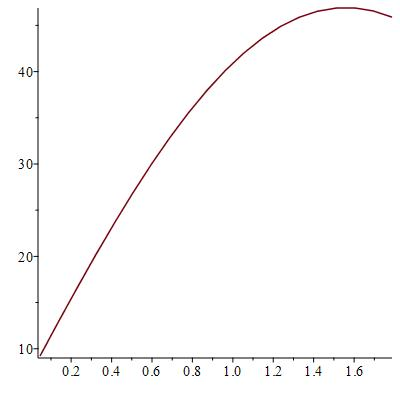
\includegraphics[width=1\linewidth]{../img/img1.jpg}}  \\
	\end{minipage}
\end{figure}
Найдем аналитическое решение уравнения

\begin{equation*}
x(s)-\frac{1}{4} \int_{0}^{\frac{11}{6}} K(s, \tau) x(\tau) d \tau=\frac{11}{6}\left(s^{2}+4\right), \quad s \in[0 ; \frac{11}{6}]
\end{equation*}

\begin{equation*}
	x(s)=C_{1} \sin (\sqrt{\frac{2(N+5)}{N(n-49)}} s)+C_{2} \cos (\sqrt{\frac{2(N+5)}{N(n-49)}} s)+(n-49)
\end{equation*}

$C_1$ и $C_2$ определим из следующей системы:

\begin{equation*}
	\left\{\begin{array}{l}{C_{2}+n-49=\frac{N+5}{N}(n-49)} \\ {C_{1} \sin \left(\sqrt{\frac{2(N+5)}{N(n-49)}} \frac{N+5}{N}\right)+C_{2} \cos \left(\sqrt{\frac{2(N+5)}{N(n-49)}} \frac{N+5}{N}\right)+(n-49)+} \\ {\frac{N+5}{N}\left[C_{1} \sqrt{\frac{2(N+5)}{N(n-49)}} \cos \left(\sqrt{\frac{2(N+5)}{N(n-49)}} \frac{N+5}{N}\right)-C_{2} \sqrt{\frac{2(N+5)}{N(n-49)}} \sin \left(\sqrt{\frac{2(N+5)}{N(n-49)}} \frac{N+5}{N}\right)\right]=} \\ {=\frac{N+5^{3}}{N}+(n-49) \frac{N+5}{N}+2 \frac{N+5}{N}}\end{array}\right.
\end{equation*}

Получаем:

\begin{equation*}
	x(s)=C_{1} \sin (\sqrt{\frac{33}{36}} s)+C_{2} \cos (\sqrt{\frac{33}{36}} s)+4
\end{equation*}

\begin{equation*}
C_1 = -{\frac {-570\,\sin \left( {\frac {19\,\sqrt {399}}{294}} \right) 
			\sqrt {399}+8820\,\cos \left( {\frac {19\,\sqrt {399}}{294}} \right) -
			59721}{532\,\cos \left( {\frac {19\,\sqrt {399}}{294}} \right) \sqrt {
				399}+8232\,\sin \left( {\frac {19\,\sqrt {399}}{294}} \right) }}
\end{equation*}

\begin{equation*}
	C_2  = \frac{15}{14}
\end{equation*}

Построим график полученного аналитического решения:

\begin{figure}[H]
	\begin{minipage}[h]{0.75\linewidth}
		\center{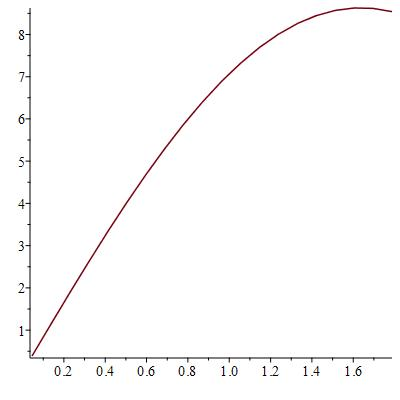
\includegraphics[width=1\linewidth]{../img/img3.jpg}}  \\
	\end{minipage}
\end{figure}


А так же построим совмещенные графики полученных решений и найдем абсолютную погрешность(красным выделено приближенное значение, синим-аналитическое решение)


\begin{figure}[H]
	\begin{minipage}[h]{1\linewidth}
		\center{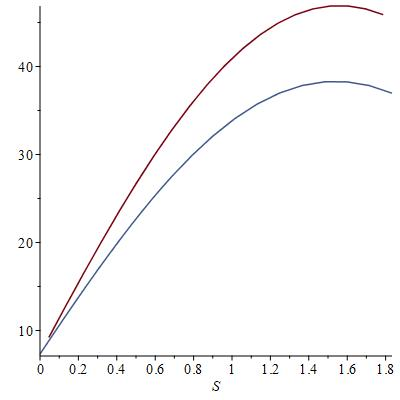
\includegraphics[width=1\linewidth]{../img/img2.jpg}}  \\
	\end{minipage}
\end{figure}

\begin{equation*}
	\Delta_{max} = 8.54122
\end{equation*}



\end{document}